\section{Quantum Dependence and the Write-All Rule}\label{sec:core}

This section defines what a slice of a set of qubits must preserve and when an operation is a dependence of
those qubits. It then states the write-all rule, proves that it gives slices that are sound and contain every
dependence, shows that three kinds of dependence are all a slice needs, and places every other rule relative to
it. The definitions do not depend on any slicer, and Section~\ref{sec:results} measures each rule against them.

\subsection{Circuits, criteria and dependence}
A Qiskit program does not act on qubits directly. It builds a \emph{circuit}, which a simulator or a quantum
computer then runs. The circuit $P = o_0 \dots o_{L-1}$ is the sequence of operations the program appends, in the
order it appends them, and position $k$ holds the operation $o_k$. The circuit has $n$ qubits, numbered
$Q = \{0, \dots, n-1\}$, which form its quantum memory, and a set $C$ of classical bits, which store the outcomes of
measurements.

Each operation touches some qubits and bits, which we call its \emph{locations} $\mathit{loc}(o) \subseteq Q \cup
C$. A gate touches the qubits it is applied to, so \texttt{h(0)} has the location $q_0$ and \texttt{cx(0, 1)} the
locations $q_0$ and $q_1$. A measurement touches the measured qubit and the bit that receives its outcome, so
\texttt{measure(2, 0)} has the locations $q_2$ and $c_0$. A reset, which returns a qubit to $\ket{0}$, touches that
qubit. A conditioned gate is applied only when a measured bit has a given value, as in \texttt{x(0)} inside
\texttt{if\_test((c[0], 1))}, and it touches its qubits and the bits its condition reads, here $q_0$ and $c_0$.

The program's own loops and branches run while the circuit is built and decide which operations it contains and
how often. Loops that run inside the circuit, on the device, are treated in Section~\ref{sec:loops}.

The state of the qubits is described by a density matrix $\rho$, which also covers the mixtures that arise when a
measurement outcome is not known in advance. Running $P$ on the input $\rho$, with every bit initially $0$, gives
$\llbracket P \rrbracket(\rho)$, the final joint state of qubits and bits, averaged over the outcomes of the
measurements. A developer asks about some of the qubits, a set $W \subseteq Q$. Their \emph{reduced state}
$\rho_W = \operatorname{Tr}_{\overline{W}}(\rho)$ is what remains of $\rho$ when everything else,
$\overline{W} = (Q \setminus W) \cup C$, is traced out, that is, averaged away. It determines every statistic of
measuring $W$ in any basis, so two runs that give $W$ the same reduced state cannot be told apart by looking at
$W$. A slice is a set $S$ of positions in $P$, and it is judged by running the restriction $P|_S$, the circuit that
keeps only the operations at the positions in $S$, in their original order.

\begin{definition}[Slicing criterion]\label{def:criterion}
A slicing criterion is a nonempty set $W \subseteq Q$ of qubits, whose state is taken at the end of the circuit,
before any terminal measurement reads it.
\end{definition}

The criterion is a set of qubits, not a single one, because a qubit has no value of its own apart from the qubits
it is correlated with. Yu and Zhao keep the classical criterion of a variable at a statement~\cite{yu2025qpdg}, and
we preserve the \emph{joint} state of the criterion instead. Taking that state before readout keeps a slice correct
when it is composed with later gates or read in another basis.

\begin{definition}[Soundness]\label{def:sound}
A set of positions $S$ \emph{preserves} $W$ at input $\rho$ if $\operatorname{Tr}_{\overline{W}}
\llbracket P|_S \rrbracket(\rho) = \operatorname{Tr}_{\overline{W}}\llbracket P \rrbracket(\rho)$. It is a
\emph{sound} slice for $W$ if it preserves $W$ at every input.
\end{definition}

A sound slice reproduces the criterion, but comprehension needs more, the assurance that the slice shows every
place where a change, and so a fault, could alter the criterion.

\begin{definition}[Dependence]\label{def:dep}
Operation $o_k$ is a \emph{dependence} of $W$ in $P$ if there are an input $\rho$ and a unitary $U$ on the qubits
of $o_k$ such that inserting $U$ immediately after $o_k$ changes $\operatorname{Tr}_{\overline{W}}\llbracket P
\rrbracket(\rho)$. For a measurement, negating the bit it writes also counts as such a change. $\mathit{Dep}_W(P)$
is the set of dependences of $W$, and a set $S$ is \emph{dependence-complete} for $W$ if $\mathit{Dep}_W(P)
\subseteq S$.
\end{definition}

This is semantic dependence in the sense of Podgurski and Clarke~\cite{podgurski1990formal}, stated for quantum
states. The two guarantees differ. A sound slice need not contain every dependence. An identity gate on a qubit
of $W$ is a dependence, since a perturbation inserted after it changes the criterion, yet deleting it changes
nothing. Conversely, deleting one unitary operation that is not a dependence never changes $\rho_W$, as
inserting its inverse shows.

\subsection{The write-all rule}
A \emph{dependence rule} $R$ assigns each operation the locations it reads, $r_R(o)$, and the locations it writes,
$w_R(o)$. Operation $o_j$ depends on $o_i$ under $R$ if $i < j$ and some location in $w_R(o_i) \cap r_R(o_j)$ is
not written by an operation between them. The backward slice $B_R(W)$ is the set of operations from which the
last writer of some $q \in W$ is reachable along these dependences. The rules differ in one choice, what an
operation writes.

\begin{definition}[Write-all rule]\label{def:writeall}
Every operation reads and writes all of its locations, $r(o) = w(o) = \mathit{loc}(o)$. In particular a
controlled gate writes its controls as well as its targets. The \emph{quantum dependence graph} (QDG) has the
operations as nodes and the dependences of this rule as edges, and the QDG slice $\Bw(W)$ is backward
reachability from $W$.
\end{definition}

The QDG slice is computed in one backward pass. Start at the end of the circuit with the needed set $N = W$, and
whenever an operation acts on a location in $N$, keep the operation and add all its locations to $N$. On qubits
alone, this is the backward light cone of $W$. The classical bits extend it, from a measurement to the
operations its bit conditions. Take the circuit
\[
P_1 \;=\; \mathrm{X}(q_1)\;\; \mathrm{H}(q_1)\;\; \mathrm{H}(q_0)\;\; \mathrm{CX}(q_0, q_1)
\]
and the criterion $\{q_0\}$. The CNOT acts on $q_0$, so it is kept and $q_1$ joins $N$, which keeps the two gates
on $q_1$ as well. Although $q_0$ is the CNOT's control, the gates on $q_1$ do change it. At input $\ket{00}$ the
target is prepared in $\ket{-}$, an eigenstate of the bit flip, so the CNOT leaves the target as it is and flips
the phase of the control, which ends in $\ket{-}$ instead of $\ket{+}$. This is phase kickback. A rule that
reads the control as unchanged lets the CNOT write only $q_1$, so the last operation to write $q_0$ is
$\mathrm{H}(q_0)$ and its slice keeps that gate alone.

\begin{theorem}[The QDG is sound]\label{thm:sound}
For every circuit $P$ and criterion $W$, $\Bw(W)$ is a sound slice for $W$.
\end{theorem}

\begin{IEEEproof}[Proof sketch]
Process $P$ backward with the needed set $N$, initially $W$. Operation $o_k$ joins the slice, and $N$ grows by
$\mathit{loc}(o_k)$, exactly when $\mathit{loc}(o_k) \cap N \neq \emptyset$, which computes $\Bw(W)$. Every gate,
reset, measurement and conditioned gate is a channel that acts only on $\mathit{loc}(o)$. By locality of the partial
trace, the no-signaling principle, an operation outside the slice cannot change the reduced state of the needed
locations after it, and an operation in the slice maps the reduced state of the needed set before it to the one
after it. Induction over $P$ gives the claim. The induction is mechanized in Isabelle/HOL for an abstract model of
local operations, and that quantum operations satisfy the model is argued on paper.
\end{IEEEproof}

\begin{proposition}[The QDG is dependence-complete]\label{prop:complete}
$\mathit{Dep}_W(P) \subseteq \Bw(W)$.
\end{proposition}

\begin{IEEEproof}
Let $o_k \notin \Bw(W)$, and let $P'$ insert a unitary $U$ after $o_k$. In the backward pass, no location of
$o_k$ is needed after it, since otherwise $o_k$ would be kept. $U$ acts only on locations of $o_k$, so $U$ is not
kept either and the needed set is unchanged. Hence $P'$ and $P$ have the same QDG slice, and by
Theorem~\ref{thm:sound} the same reduced state of $W$. A negated outcome is handled alike, as an operation on the
bit of a measurement outside the slice.
\end{IEEEproof}

\begin{proposition}[The QDG distributes over criteria]\label{prop:joint}
$\Bw(W_1 \cup W_2) = \Bw(W_1) \cup \Bw(W_2)$.
\end{proposition}

\begin{IEEEproof}
In the backward pass of Theorem~\ref{thm:sound}, the needed set for $W_1 \cup W_2$ is at every position the union
of those for $W_1$ and $W_2$.
\end{IEEEproof}

Together these say that the QDG slice is exactly what a slice must keep. It keeps everything that can change the
criterion and reproduces the criterion for every input, and the slice of a set of qubits is the union of the slices
of its members, so a tool computes single-qubit slices and combines them. The relation itself is not new. It is the
light cone that compilers compute, and LintQ orders operations by it~\cite{paltenghi2024lintq}. What the three
results add is the justification of that relation as a slice.

\paragraph*{Why the write set cannot be smaller}
Dropping a qubit from the write set of a two-qubit gate is safe only if that gate can never carry information from
the other qubit to it. No standard gate qualifies. For each of the \numGateSignalN{} two-qubit gates of Qiskit's
standard library, from the CNOT and CZ to the SWAP and the parameterized rotations, a change of either qubit's input
changes the reduced state of the other for some product input (exploratory, Deviation I-24). A rule that reads any
of these gates as writing only some of its qubits therefore misses a dependence of some circuit.
% TODO authors: a general necessity proposition (every two-qubit gate that is not a product of single-qubit gates
% signals in both directions) needs checking against Beckman et al., Phys. Rev. A 64 (2001), before it is stated.

\subsection{Three kinds of dependence suffice}\label{sec:kinds}
The write-all rule needs only three kinds of dependence, which Table~\ref{tab:kinds} lists with examples from the
ansatz of Fig.~\ref{fig:ansatz}. \emph{Classical data} dependence follows the host values that compute gate
arguments, such as angles, sizes and qubit indices. \emph{Classical control} dependence follows what decides
whether an operation is applied at all. It covers the host program's loops and branches, which decide when the
circuit is built which operations it contains and how often, and the measured bits that condition operations when
the circuit runs, in a conditioned gate, a branch or a loop of the circuit. \emph{Quantum data} dependence follows
a qubit through the operations that act on it, under the write-all rule.

A controlled gate looks like a fourth kind, quantum control dependence, since it reads like a branch, if the control
is 1 then flip the target. It is not one. Its control is coherent, so the gate acts on a superposition of control
values and no branch is ever taken, and it can change its control, as $P_1$ shows. What looks like control
dependence is quantum data dependence in both directions, which the write-all rule records, and reading the gate as
a branch is exactly the error of the classical PDG in Section~\ref{sec:rules}. Real control dependence in a quantum
program arises only through measurement, whose classical bit then conditions later operations.

\begin{table}[t]
  \centering
  \caption{The kinds of dependence a quantum slice needs}
  \label{tab:kinds}
  \footnotesize\setlength{\tabcolsep}{3pt}\renewcommand{\arraystretch}{1.15}
  \begin{tabular}{@{}>{\raggedright\arraybackslash}p{1.55cm} >{\raggedright\arraybackslash}p{3.2cm}
                  >{\raggedright\arraybackslash}p{3.15cm}@{}}
    \toprule
    \textbf{Kind} & \textbf{Follows} & \textbf{In Fig.~\ref{fig:ansatz}a} \\
    \midrule
    Classical data & host values that compute gate arguments & \texttt{n}, \texttt{layers}, the angles \\
    \arrayrulecolor{black!25}\hline\arrayrulecolor{black}
    Classical control & host loops and branches, and measured bits that condition operations & \texttt{for qubit in range(n)}, the flip conditioned on the measured bit \\
    \arrayrulecolor{black!25}\hline\arrayrulecolor{black}
    Quantum data & every qubit an operation acts on, written by the write-all rule & \texttt{cx(qubit, qubit+1)} writes both qubits \\
    \midrule
    Quantum control & no kind of its own, it is quantum data dependence & a controlled gate is not a branch \\
    \bottomrule
  \end{tabular}
\end{table}

The other kinds proposed for quantum programs add no dependence either. Entanglement is the most natural
candidate, since entangled qubits are correlated, but it decides nothing.

\begin{proposition}[Entanglement is neither necessary nor sufficient for dependence]\label{prop:ent}
(i) An operation can be a dependence of $q$ although, at an input that witnesses the dependence, $q$ is never
entangled with its qubits. (ii) An operation can act on a qubit entangled with $q$ and not be a dependence of $q$.
\end{proposition}

\begin{IEEEproof}
(i) In $P_1$ at input $\ket{00}$, the state is a product state after every operation, yet the gates on $q_1$ are
dependences of $q_0$, since inserting $\mathrm{H}(q_1)$ after them changes the final state of $q_0$. (ii) In
$\mathrm{H}(q_0)\,\mathrm{CX}(q_0, q_1)\,\mathrm{X}(q_1)$ the two qubits are maximally entangled before
$\mathrm{X}(q_1)$, but by no-signaling no operation on $q_1$ after the CNOT can change $\rho_{q_0}$.
\end{IEEEproof}

By Proposition~\ref{prop:complete}, entanglement edges can add no dependence that the QDG misses, and by (ii) they
can add operations that are not dependences. The remaining proposed kinds add no edges. A CNOT that copies a basis
state, the case no-cloning concerns, is a two-qubit gate whose edges quantum data dependence already has. Timing
decides when an operation runs on hardware, not what a state depends on, and a compiler can move a single-qubit
gate within the idle time of its qubit without changing the ideal computation~\cite{smith2022timestitch}.
Superposition changes amplitudes, not which locations an operation acts on~\cite{nielsen2010quantum}, so it cannot
add an edge to a dependence graph.

\subsection{The other rules, relative to the write-all rule}\label{sec:rules}
The study compares the write-all rule with the rules a developer or tool builder would otherwise use.
Table~\ref{tab:rules} gives each by how it differs from the QDG, and Fig.~\ref{fig:ansatz} applies them to one
program that needs every kind of dependence. An ansatz is the parameterized circuit of a variational algorithm,
whose rotation angles a classical optimizer tunes. The ansatz of Fig.~\ref{fig:ansatz}a has layers of rotations and
a chain of CNOTs, and after them an auxiliary qubit is measured mid-circuit and $q_0$ is flipped when the outcome
is~$1$.

\begin{figure*}[t]
  \centering
  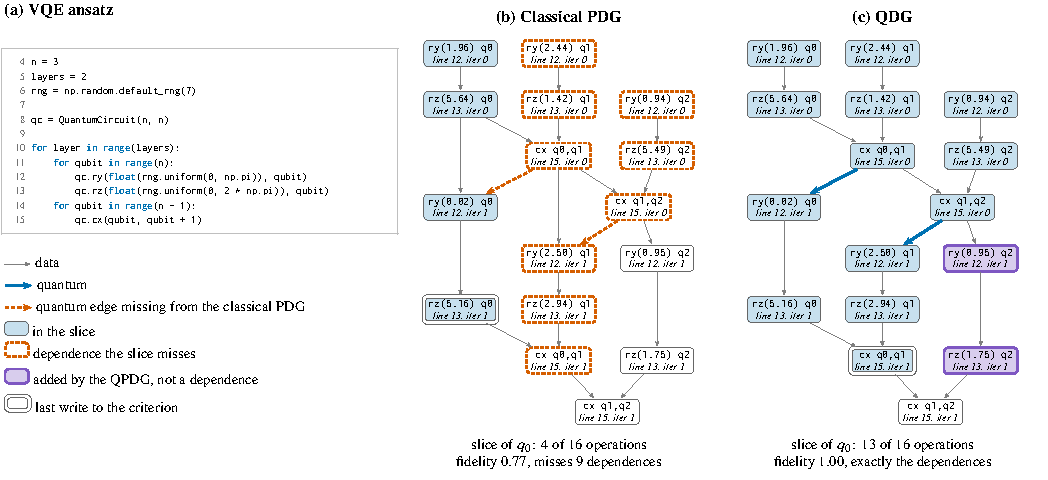
\includegraphics[width=\textwidth]{figures/fig_pdg_ansatz.pdf}
  \caption{The rules on a variational ansatz, criterion $q_0$. (a)~The program. After the loops, an auxiliary qubit
  is measured mid-circuit and conditions a flip of $q_0$. (b)~One graph for the first four rules of
  Table~\ref{tab:rules}. Each node is an operation as it executes, with its source line and loop iteration, and a box
  holds each iteration of the outer loop. Grey data edges belong to every rule, and def-use lacks the green control
  edge from the measurement. The classical PDG and def-use lack the blue quantum edges and have the dotted edges
  instead, each of which skips a CNOT whose control it reads as unchanged. A node is shaded by the weakest rule that
  keeps it. The QDG keeps exactly the dependences of $q_0$, and the QPDG adds the hatched operations, which are not
  dependences. Graphs, slices and fidelities at $\ket{0\dots0}$ are computed by the study's code from the program
  shown.}
  \label{fig:ansatz}
\end{figure*}

\begin{table}[t]
  \centering
  \caption{The dependence rules, by what a CNOT with control $c$ and target $t$ writes and by how each differs from
  the QDG}
  \label{tab:rules}
  \footnotesize\setlength{\tabcolsep}{2.6pt}\renewcommand{\arraystretch}{1.12}
  \begin{tabular}{@{}l c >{\raggedright\arraybackslash}p{2.05cm} >{\raggedright\arraybackslash}p{1.38cm} r r@{}}
    \toprule
    \textbf{Rule} & $w(\mathit{cx}_{c,t})$ & \textbf{Relation to the QDG} & \textbf{Guarantee} & \textbf{Ops} & $F$ \\
    \midrule
    \rowcolor{blue!7}\textbf{QDG} & $\{c, t\}$ & \textbf{write-all rule} & \textbf{sound, complete} & \numAnsWireOps{} & \numAnsQdgFidelity{} \\
    \midrule
    Def-use & $\{t\}$ & $-$ control write, $-$ bits & none & \numAnsDuOps{} & \numAnsDuFidelity{} \\
    Classical PDG & $\{t\}$ & $-$ control write & none & \numAnsCpdgOps{} & \numAnsCpdgFidelity{} \\
    QPDG~\cite{yu2025qpdg} & $\{c, t\}$ & $+$ closed entanglement edges & sound & \numAnsYzOps{} & \numAnsYzFidelity{} \\
    QPDG, read-only & $\{t\}$ & $-$ control write, $+$ entanglement & none & \numAnsYzroOps{} & \numAnsYzroFidelity{} \\
    \bottomrule
  \end{tabular}\\[3pt]
  \begin{minipage}{\columnwidth}\footnotesize
  Every rule reads $\{c, t\}$, and complete means dependence-complete. Commutation and state-based pruning remove
  operations from the QDG slice. Ops is the number of the \numAnsOps{} operations of Fig.~\ref{fig:ansatz} that the
  slice of $q_0$ keeps, and $F$ its fidelity at $\ket{0\dots0}$.
  \end{minipage}
\end{table}

\paragraph*{The classical PDG and def-use}
The classical PDG, written CPDG in subscripts, applies the program dependence graph~\cite{ferrante1987pdg} to the
circuit. It reads a gate as a classical assignment, so a controlled gate reads its controls and targets and writes
only its targets, and any other gate reads and writes all its qubits. A measurement writes its bit, and a
conditioned gate reads the bits its condition tests. \emph{Def-use} (DU) is the same data dependence without the
bits, the simplest transfer of classical slicing. Reading a control as unchanged is the usual explanation of a
CNOT~\cite{ramalho2025road}, and it holds for computational basis states. A table of the operations on each qubit
that marks the control of a CNOT apart from its target~\cite{behler2024supporting} serves pattern detection well,
but read as a dependence graph it gives this reading.

\begin{proposition}[The classical PDG is unsound]\label{prop:du}
There are circuits for which neither $B_{\mathrm{CPDG}}(W)$ nor $B_{\mathrm{DU}}(W)$ preserves $W$, even at
$\ket{0\dots0}$.
\end{proposition}

The ansatz of Fig.~\ref{fig:ansatz} is a witness for both, and on unitary circuits the two slices are equal.
Def-use ignores the classical bits, so its slice of $q_0$ keeps only \numAnsDuOps{} of the \numAnsOps{} operations,
with fidelity \numAnsDuFidelity{}, and loses the auxiliary's gate and measurement, which the classical PDG reaches
through the green control edge in Fig.~\ref{fig:ansatz}b. Control dependence is not enough, however. Each
\texttt{cx(qubit, qubit+1)} changes its control as well as its target, so the state of $q_0$ comes to depend on the
rotations of $q_1$ and, from the second layer on, of $q_2$. The classical PDG keeps only \numAnsCpdgOps{}
operations, misses \numAnsCpdgMissed{} dependences and reaches fidelity \numAnsCpdgFidelity{}. Where the QDG has
a blue quantum edge out of a CNOT, the classical PDG has a dotted edge that skips the CNOT. The QDG slice keeps the
\numAnsWireOps{} operations that are dependences of $q_0$, and no other.

\paragraph*{The QPDG}
Our reimplementation of Yu and Zhao's graph~\cite{yu2025qpdg} serves as a baseline. Its dependences are given in
prose, so we logged every reading of it before any run. Data and control dependence are as in the QDG. The QPDG
gives no rule for when two qubits are entangled, so we use the flow-insensitive rule of entanglement analysis, under
which qubits joined by a two-qubit gate anywhere in the circuit are entangled~\cite{javadiabhari2015scaffcc}, and
add an edge from every operation to every later one on qubits of the same component. A flow-sensitive variant
counts two qubits as entangled only from the first gate that couples them. Either way the QPDG is the QDG plus
entanglement edges, so its slices contain those of the QDG, and in Fig.~\ref{fig:ansatz}b the extra edges add the
\numAnsYzExtra{} hatched operations of $q_2$ in the second layer, which run after the last gate that carries
information from $q_2$ to $q_0$. Yu and Zhao do not say whether a gate writes its control, so we also run, as an
exploratory variant, the reading in which it does not.

\paragraph*{Pruning}
Two refinements start from the QDG slice and remove operations from it. \emph{Commutation pruning} propagates the
Pauli observables $X$, $Y$ and $Z$ of every criterion qubit backward and removes each operation that commutes with
all of them, since such an operation cannot change a measurement statistic of the criterion. Qiskit's
\texttt{LightCone} pass implements it~\cite{qiskit2025}. \emph{State-based pruning} fixes one input, by default
$\ket{0\dots0}$, and removes an operation that does not act on the criterion if the mutual information between the
criterion and the operation's qubits is below $10^{-9}$ and the removal still preserves $W$ at that input. Both give
smaller slices, but neither is dependence-complete, and a state-based slice holds for its one input only, as a
conditioned slice does~\cite{canfora1998conditioned}.

\subsection{Loops}\label{sec:loops}
A loop of the host program runs when the circuit is built. A static slicer unrolls it, so every iteration
contributes its own operations, each tagged with the line and iteration that emit it. When the number of iterations
cannot be known statically, the loop body is repeated as \emph{may-operations}, operations that might be emitted,
until no repetition adds a location to any dependence chain. A loop of the circuit itself, Qiskit's
\texttt{while\_loop}, \texttt{for\_loop} or \texttt{switch}, runs on the device, and its condition reads measured
bits. Its body is treated the same way, with every operation in it conditioned on the bits its condition reads, so
the classical control dependence on the measurement that decides the loop is kept.

\begin{proposition}[Loops]\label{prop:loops}
Let a loop body $B$ act on a set of locations $\Lambda$, let the loop end with probability one, and let $P_B$ repeat
$B$ $|\Lambda| + 1$ times, with every operation of $B$ conditioned on the bits that decide the loop. Deleting from
$B$ every operation that no copy in the QDG slice of $P_B$ keeps gives a sound slice for every criterion.
\end{proposition}

\begin{IEEEproof}[Proof sketch]
A loop that runs at most $K$ times is the circuit of $K$ copies of $B$, each conditioned on the bits that decide
the loop, a circuit with conditioned operations to which Theorem~\ref{thm:sound} applies. In its backward pass every
copy is processed alike, and the needed set only grows. Once a copy adds no location of $\Lambda$, every earlier copy
keeps the same operations, and the needed set can grow at most $|\Lambda|$ times, so for every $K$ the copies keep
only operations that one of the $|\Lambda| + 1$ copies of $P_B$ keeps. The bits that decide the loop are read by
every copy, so the measurements that write them are kept and the distribution over numbers of iterations is
preserved. A loop that ends with probability one is the limit of its bounded prefixes.
\end{IEEEproof}

The induction of Theorem~\ref{thm:sound} is not mechanized for loops, and the proposition is argued on paper. It is
checked exactly on \numCfPrograms{} programs of our own with circuit loops, branches and switches. For every one of
their \numCfQubits{} qubits, deleting every operation outside the qubit's slice from the source leaves the qubit's
state unchanged at \numCfInputs{} inputs, while the slices that read a circuit loop's body once are wrong on
\numCfOldWrong{} of the \numCfPrograms{} programs (exploratory, Deviation I-26).

\subsection{Forward slices and qubit profiles}
The forward slice $\Fw(o_k)$ of an operation is the set of operations reachable from $o_k$ in the QDG. It answers
the question a developer asks before changing a gate, which later operations and qubits the change can reach. We say
that $o_k$ reaches $q$ if $\Fw(o_k)$ contains the last operation on $q$.

\begin{proposition}[Forward and backward slices are dual]\label{prop:dual}
For every operation $o_k$ and qubit $q$, $o_k$ reaches $q$ if and only if $o_k \in \Bw(\{q\})$. Hence $o_k$ reaches
every qubit of which it is a dependence.
\end{proposition}

\begin{IEEEproof}
Both sides say that the QDG has a path from $o_k$ to the last operation on $q$. The second claim follows from
Proposition~\ref{prop:complete}.
\end{IEEEproof}

A slice can be reported as operations, loop iterations or source lines. Operations are the unit of the definitions
and lines the unit of the developer. A line is in a slice if one of its operations is, so a line can be kept for
one iteration only. In the second layer of the ansatz, the rotations of $q_2$ are not dependences of $q_0$, yet
their lines are in its slice because their first-layer iterations are. A line slice therefore names the iterations
that put each line in it.

The slice profile of a variable, which srcSlice records~\cite{alomari2014srcslice}, has a quantum counterpart that
gathers in one view what a developer first asks about a qubit.

\begin{definition}[Qubit slice profile]\label{def:profile}
The profile of a qubit $q$ records its \emph{uses}, the lines of the operations on $q$, each of which both reads
and writes $q$ under the write-all rule; its \emph{names}, the source expressions that denote $q$ in gate calls; its
\emph{functions}, the call sites of the functions in which $q$ is acted on; its \emph{dependents}, the qubits that the
first operation on $q$ reaches; its \emph{bits}, those measured from $q$, with the lines they condition; and its
\emph{backward} and \emph{forward} entries, the lines of the backward slice of $q$ and of the forward slice of its
first operation.
\end{definition}
